\chapter{Usage Guide}

\label{chap:usage_guide}



This section is aimed at describing the general use of the software, since it is
\textbf{deployed, configured} and \textbf{run}.

This software is used by actors. These actors rely on the software to perform a
set of business activities (called here procedures) aimed at reaching a
particular goal. 

These prodedures are splet in two groups:
\begin{itemize}
  \item \textbf{Multi-procedures:} which are procedures at \textbf{summary} or
  \textbf{user-goal} level involving several active or pro-active actors.
  Each of these procedures aims at illustrating intertwined
  business activities required to be performed by the involved actors
  to reach the expected goal. Each business activity between the system and an
  actor must correspond to a \textbf{system operation} instance given with actual parameter values.

  \item \textbf{Mono-procedures:} which are procedures at \textbf{summary} or
  \textbf{user-goal} level involving only one active or pro-active actor.
  Each of these procedures aims at illustrating the required business
  activities an actor has to perform to reach the expected goal. Each business
  activity between the system and the actor must correspond to a \textbf{system
  operation} instance given with actual parameter values.

\end{itemize}



Each process has to be documented using the following textual description
template \cite{armour01usecase} \textbf{BUT its content must be as low level as possible with actual values}:

\vspace{0.5cm}

\hrule
\begin{lyxlist}{PC1}

\small{

\item [\textbf{Procedure:}] ProcessMissionOne
\item [\textbf{Scope:}] Crisis Management System (\emph{CMS})
\item [\textbf{Primary Actor}:] Coordinator John
\item [\textbf{Secondary Actor(s)}:] FirstAidWorker Bob,\\
                  ExternalResourceSystem ERS
\item [\textbf{Goal:}] The intention of the Coordinator is to process mission
with ID equal to 1.
\item [\textbf{Level}:] User-goal level
\item [\textbf{Main~Success~Scenario}]:\\
1. \emph{John} instructs the \emph{CMS} to process the mission with ID equal to 12.031005\\
2. \emph{CMS} selects the internal worker \emph{Bob} to execute the mission 12.031005\\
3. \emph{CMS} instructs \emph{Bob} to behave as \emph{First Aid Worker (FAW)}\\
4. \emph{Bob} informs the \emph{CMS} of his arrival\\
5. \emph{Bob} informs the \emph{CMS} that he starts to execute the mission 12.031005\\
6. \emph{Bob} informs the \emph{CMS} that the mission 12.031005 outcome is ``Mission completed''


\item [\textbf{Extensions}]:\\
2.a None internal worker can execute the mission\\
\hspace*{0.5cm} 2.a.1 \emph{CMS} sends a request for an external resource to the \emph{ERS} actor instance\\
\hspace*{0.5cm} 2.a.2 \emph{ERS} informs \emph{CMS} that the request can be processed\\
\hspace*{0.5cm} 2.a.3 \emph{ERS} informs \emph{CMS} that \emph{Bob} can now be selected as first aid worker\\
\hspace*{0.5cm} \textbf{procedure continues at step 3}

}

\end{lyxlist}
\hrule
\vspace{0.5cm}




\Remark{Processes presentation}: processes should be introduced to the
reader in a pedagogical manner. Thus, simple and common processes should be presented before
than more complex and less utilised ones.

\Remark{Graphical User Interfaces (GUIs)}: include GUIs screenshots to show the
different stages of the process while its is performed by the actor(s).






\section{Multi-procedures}


\subsection{Ask for diffrent fruit or vegtable}
\vspace{0.5cm}
\hrule
\hfill \break
\begin{lyxlist}{PC1}
\small{
\item [\textbf{Procedure:}] Ask for a diffrent fruit or vegtable
\item [\textbf{Scope:}] New fruit or vegtable demand to the manager.
\item [\textbf{Primary Actor}:] Gardener
\item [\textbf{Secondary Actor(s)}:] Manager
\item [\textbf{Goal:}] The intention that the gardner can ask a new Fruit or
Vegtable to the manager and to show to the manager the demand.
\item [\textbf{Level}:] User-goal level
\item [\textbf{Main~Success~Scenario}]:\\
1. \emph{Gardner} Complets the diffrent text fields with there given
information and presses the button \emph{Ask to the manager}. \\
2. Shows a pop up with the information entred.\\
3. \emph{Gardner} Has to choice to accept or to cancel .\\
	3.a \textbf{In case of accept:}
		\begin{Tab}{2em}  requested item send to the manager.\end{Tab}
	3.b \textbf{In case of decline:}
		\begin{Tab}{2em} \emph{System} cancels the action and the gardner can
		now refill the input or do an other task. \end{Tab}
\item [\textbf{Extensions}]:\\
2.a  \emph{Manager} Approves the request or declines the request.\\
}
\end{lyxlist}
\hrule
\vspace{0.5cm}






\subsection{Remove crops from inventory}

\vspace{0.5cm}
\hrule
\hfill \break
\begin{lyxlist}{PC1}
\small{
\item [\textbf{Procedure:}] Possibility to remove an hole inventory of crops.
\item [\textbf{Scope:}] Deletes all the Crops left of one kind from the table.
\item [\textbf{Primary Actor}:] Manager
\item [\textbf{Secondary Actor(s)}:] Software
\item [\textbf{Goal:}] The intention that the manager can delet an hole stock of
crops for any reason.
\item [\textbf{Level}:] User-goal level
\item [\textbf{Main~Success~Scenario}]:\\
1. \emph{Manager} is on the manager screen. \\
2. \emph{Manager} sees the inventory table.\\
3. \emph{Manager} by pressing the red button he cant delete the given row of
crops.\\
4. \emph{System} shows up a message of success and table gets updated.
5. \emph{System} updates the Gardner inventory table.
\item [\textbf{Extensions}]:\\
2.a  \emph{System} sends a message or a nodentification to the gardner that a
change has been done to the inventory table.\\
}
\end{lyxlist}
\hrule
\vspace{0.5cm}




\break


\subsection{Sign In}
\vspace{0.5cm}
\hrule
\hfill \break
\begin{lyxlist}{PC1}
\small{
\item [\textbf{Procedure:}] SignIn
\item [\textbf{Scope:}] Identified usage of the software
\item [\textbf{Primary Actor}:] User
\item [\textbf{Secondary Actor(s)}:] Greenhouse Software GS
\item [\textbf{Goal:}] Show the user GUI to manage the garden
\item [\textbf{Level}:] User-goal level
\item [\textbf{Main~Success~Scenario}]:\\
1. \emph{User} enters a username and password combination and signs in\\
2. \emph{GS} looks up the user rights defined by the administrator\\
3. \emph{GS} now show the correct Graphical User Interface (GUI) \emph{(Gardener, Technician, Manager or Administrator)} able to control the garden.
\item [\textbf{Extensions}]:\\
1.a Wrong username and password combination\\
\hspace*{0.5cm} 1.a.1 \emph{GS} notifies the \emph{User} that the entered information are wrong\\
\hspace*{0.5cm} \textbf{procedure recontinues at step 1}
}
\end{lyxlist}
\hrule
\vspace{0.5cm}


\subsection{Adding task to the gardeners schedule}
\vspace{0.5cm}
\hfill \break
\hrule
\begin{lyxlist}{PC1}
\small{
\item [\textbf{Procedure:}] Adding data to a datalist
\item [\textbf{Scope:}] Adding a task to the schedule
\item [\textbf{Primary Actor}:] actManager
\item [\textbf{Secondary Actor}:] actSystem
\item [\textbf{Goal:}] Manager can add a task to the schedule
\item [\textbf{Level}:] User-goal level
\item [\textbf{Main~Success~Scenario}]:\\
1. \emph{actManager} presses the add button\\
2. \emph{actSystem} adds task to data list\\
}
\end{lyxlist}
\hrule
\vspace{0.5cm}

\break

\subsection{Gardener searches a task in the gardeners schedule}
\vspace{0.5cm}
\hrule
\hfill \break
\begin{lyxlist}{PC1}
\small{
\item [\textbf{Procedure:}] Searching data list for matching data
\item [\textbf{Scope:}] Searching schedule for a specific task
\item [\textbf{Primary Actor}:] actGardener
\item [\textbf{Secondary Actor}:] actSystem
\item [\textbf{Goal:}] actGardener can access the gardeners schedule
\item [\textbf{Level}:] User-goal level
\item [\textbf{Main~Success~Scenario}]:\\
1. \emph{actManager} presses the search button\\
2. \emph{actSystem} will search the data list for matching data\\
\item [\textbf{Extensions}]:\\
2.a No matching data found\\
\hspace*{0.5cm} 2.a.1 \emph{actSystem} will display an empty data list}
\end{lyxlist}
\hrule
\vspace{0.5cm}



\break



\section{Mono-procedures}



\subsection{Technician}

\subsubsection{Ask for new sensor}

\vspace{0.5cm}
\hrule
\hfill \break
\begin{lyxlist}{PC1}
\small{
\item [\textbf{Procedure:}] AskForNewSensor
\item [\textbf{Scope:}] New Sensor demand to the manager.
\item [\textbf{Primary Actor}:] Technician
\item [\textbf{Goal:}] The intention that the technician can ask a new Sensor to
the manager and to show to the manager the demand.
\item [\textbf{Level}:] User-goal level
\item [\textbf{Main~Success~Scenario}]:\\
1. \emph{Gardner} complets the diffrent text fields with there given
information and presses the button \emph{push to the manager}. 
\begin{figure}
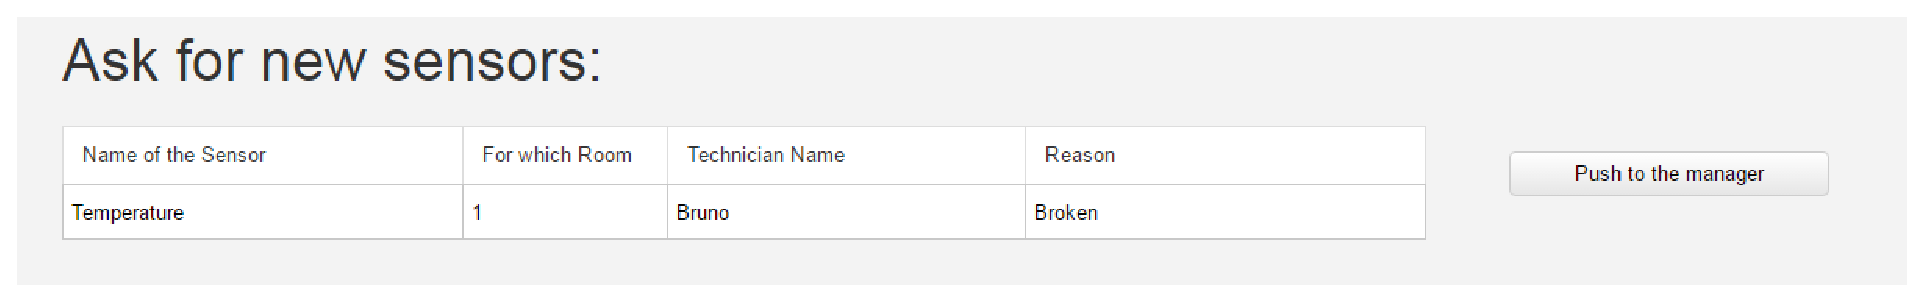
\includegraphics[width=1\textwidth]{images/AskForNewSensor.eps}
\end{figure} \\
2. Message appears of validation.
 \begin{figure}
\includegraphics[width=1\textwidth]{images/RequestAskForNewSensor.eps}
\end{figure}
\item [\textbf{Extensions}]:\\
2.a  \emph{Manager} sends to the Gardner a message of
validation or not.\\
}
\end{lyxlist}
\hrule
\vspace{0.5cm}

\break

\subsubsection{Add a new sensor to a room}
\vspace{0.5cm}
\hrule
\hfill \break
\begin{lyxlist}{PC1}
\small{
\item [\textbf{Procedure:}] AddaNewSensor
\item [\textbf{Scope:}] Adding a sensor to a room.
\item [\textbf{Primary Actor}:] Technician
\item [\textbf{Goal:}] The intention to add a sensor to a specifique room.
\item [\textbf{Level}:] User-goal level
\item [\textbf{Main~Success~Scenario}]:\\
1. \emph{Gardner} complets the diffrent text fields with there given
information and presses the green plus button. 

 \begin{figure}
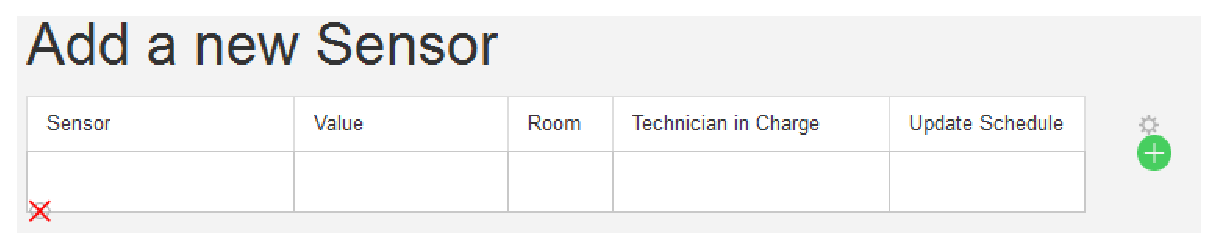
\includegraphics[width=1\textwidth]{images/AddANewSensor.eps}
\end{figure} 
2. Message appears of validation.
 \begin{figure}

\includegraphics[width=1\textwidth]{images/RequestAddANewSensor.eps}
\end{figure}
\item [\textbf{Extensions}]:\\
2.a  \emph{Manager} gets notified where the new sensor is positioned .\\
}
\end{lyxlist}
\hrule
\vspace{0.5cm}




\subsection{Manager}
\subsubsection{Add Room}

\vspace{0.5cm}
\hrule
\hfill \break
\begin{lyxlist}{PC1}
\small{
\item [\textbf{Procedure:}] Add a new room the database
\item [\textbf{Scope:}] Ability to add more rooms if needed.
\item [\textbf{Primary Actor}:] Manager
\item [\textbf{Goal:}] The manager is able to add rooms to the database.
\item [\textbf{Level}:] User-goal level
\item [\textbf{Main~Success~Scenario}]:\\
1. \emph{Manager} is on the settings screen. \\
2. \emph{Manager} fills in all data for the room (RoomName = 'Room 1', Width
= 5, Length = 3, SoilHeight = 0,5).\\
3. \emph{Manager} clicks on the \emph{Add Room} button.
}
\end{lyxlist}
\hrule
\vspace{0.5cm}
\break




\subsubsection{Delete Room}

\vspace{0.5cm}
\hrule
\hfill \break
\begin{lyxlist}{PC1}
\small{
\item [\textbf{Procedure:}] Deletes a room from the database
\item [\textbf{Scope:}] Ability to remove rooms if needed.
\item [\textbf{Primary Actor}:] Manager
\item [\textbf{Goal:}] The manager is able to remove rooms from the database.
\item [\textbf{Level}:] User-goal level
\item [\textbf{Main~Success~Scenario}]:\\
1. \emph{Manager} is on the settings screen. \\
2. \emph{Manager} clicks on the red remove button to delete the selected room.
}
\end{lyxlist}
\hrule
\vspace{0.5cm}
\break




\subsubsection{Requests for fruit or vegtable}

\vspace{0.5cm}
\hrule
\hfill \break
\begin{lyxlist}{PC1}
\small{
\item [\textbf{Procedure:}] Possibility to accept or decline a requested fruit
or vegtable.
\item [\textbf{Scope:}] Ability to accept the request from the system or the
gardner.
\item [\textbf{Primary Actor}:] Manager
\item [\textbf{Goal:}] The intention that the manager can decline or accept a
given vegtable or fruit request.
\item [\textbf{Level}:] User-goal level
\item [\textbf{Main~Success~Scenario}]:\\
1. \emph{Manager} is on the manager request screen. \\
2. \emph{Manager} sees the request fruit or vegtable table.\\
3. \emph{Manager} has to choice red cross or green arrow button.\\
3.a \textbf{In case of the green button:}
 \begin{Tab}{2em} 3.a.1 Message appears of validation and that the request
 has been validated and refilled.\\
  \end{Tab}
3.b \textbf{In case of the red button}
\begin{Tab}{2em} 3.b.1 The request is removed from the table.\\
3.b.2 The decline won't work if there is no decline.
\end{Tab}
}
\end{lyxlist}
\hrule
\vspace{0.5cm}
\break




\subsection{Gardener}
\subsubsection{Retrive/Modify Crops from Table}

\vspace{0.5cm}
\hrule
\hfill \break
\begin{lyxlist}{PC1}
\small{
\item [\textbf{Procedure:}] Retrives vegtable or
frood the amount left of crops
\item [\textbf{Scope:}] Retrives Crops from the table or asks for new non
existing items.
\item [\textbf{Primary Actor}:] Gardener
\item [\textbf{Goal:}] The intention that the gardner can retrive he's desired
amount of crops from the storage of crops to plant the crops or ask for a
diffrent frood or vegtable.
\item [\textbf{Level}:] User-goal level
\item [\textbf{Main~Success~Scenario}]:\\
1. \emph{Gardner} Complets the diffrent text fields with there given
information and presses the button \emph{Modify}. \\
\begin{figure}
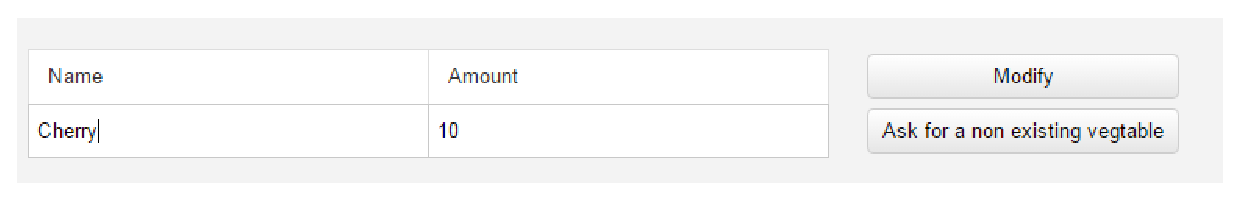
\includegraphics[width=1\textwidth]{images/RetriveCropsBase.eps}
\end{figure}
2.A pop up appears with the previsualisation of the information entred.\\
\begin{figure}
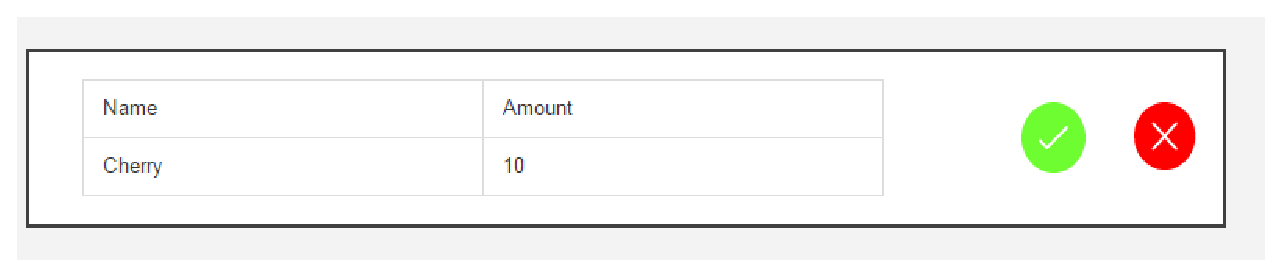
\includegraphics[width=1\textwidth]{images/PopUpRetrive.eps}
\end{figure}
3. \emph{Gardner} Has the choice to accept or to cancel .\\
	3.a \textbf{In case of accept green button:}
		\begin{Tab}{2em}  the request has been passed to the manager.\end{Tab}
	3.b \textbf{In case of decline red button:}
		\begin{Tab}{2em} cancels the action and the gardner can
		now refill the input or do an other task. \end{Tab}
\item [\textbf{Extensions}]:\\
2.a  \emph{Manager} Approves the request or declines the request.\\
}
\end{lyxlist}
\hrule
\vspace{0.5cm}

\ldots

\subsubsection{MyProcedure2MyActor2}
\ldots














